\section{Knotenpunktregel}\label{knotenpunktregel}

\subsection{Beispiel 1}\label{beispiel-1}

Für den untenstehenden Knoten ist der zeitliche Verlauf der drei Ströme
\(I_1 = f(t)\), \(I_2 = f(t)\) und \(I_3 = f(t)\) bekannt. Zeichne den
fehlenden Strom \(I_4\) auf.\\

\begin{tikzpicture}
    \draw 
    (0,3) to[short, i=$i_1$, -*] (2,2)
    (2,2) to[short, i=$i_2$] (0,0)
    (2,2) to[short, i=$i_3$] (4,4)
    (2,2) to[short, i=$i_4$] (5,2);
\end{tikzpicture}

\begin{figure}[htbp]
\centering
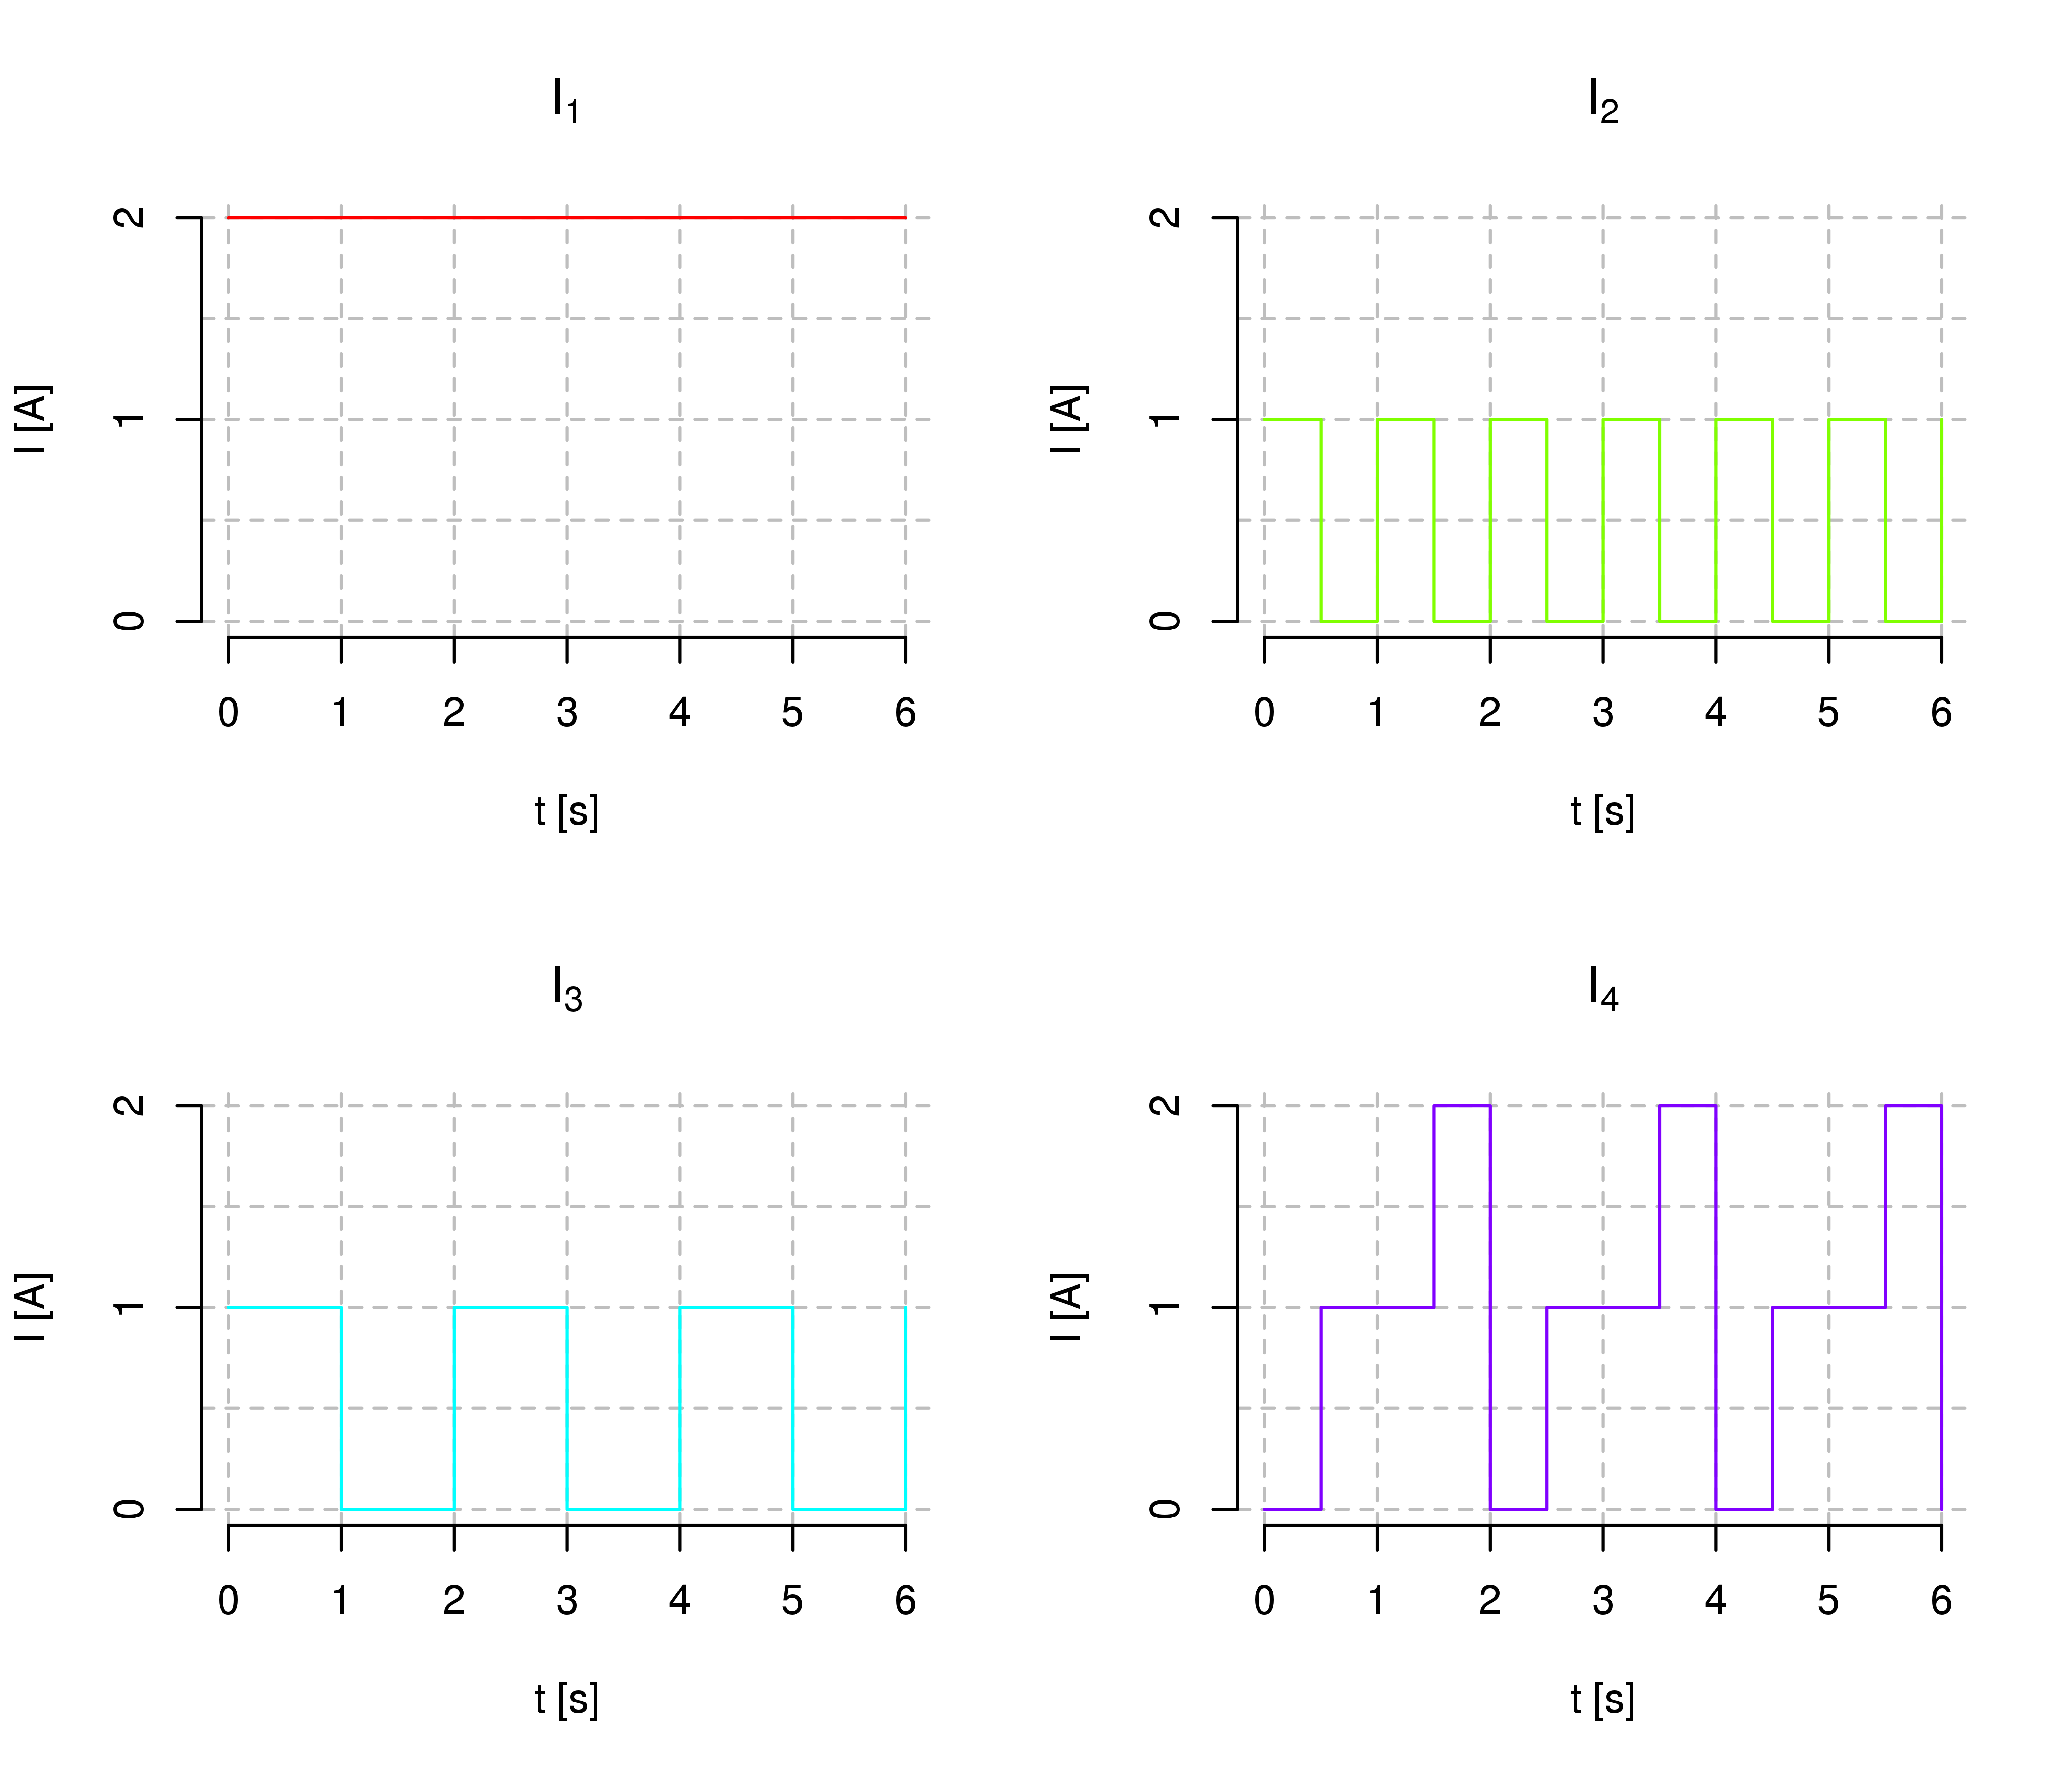
\includegraphics{img/kirchhoff_1-1.png}
\caption{Stromverlauf}
\end{figure}
